\chapter{Supplementary material for \autoref{chap:rys}}
\section{Materials and methods}
\subsection{Zebrafish husbandry}
Zebrafish husbandry was performed as described in \autoref{ssec:husbandry}.

\subsection{Generation of transgenic vsx2:eGFP \textit{rys} line}
\autoref{progenitoridentity} makes use of coronal cryosections of \textit{Tg(vsx2:eGFP)} \textit{rys} animals. Transgenesis was performed using reagents from the Tol2kit \cite{Kwan2007}, which uses the Invitrogen Gateway plasmid construction system to assemble three-part constructs from donor plasmids. Briefly, the Gateway system uses BP clonase to introduce fragments of interest into sets of 3 entry vectors, which are recombined in predictable order by LR clonase. Tol2kit consists of a numbered, standardized set of preconstructed entry vectors intended for use in the construction of transposable Tol2 transgenesis vectors.

The construct of interest was built from a $\sim$1.1kb fragment of the 5' promoter sequence of vsx2 in the 5' entry vector, an eGFP expression cassette in the middle entry vector (Tol2kit \#383), and a polyadenylation signal in the 3' entry vector (Tol2kit \#302), recombined into pdestTol2pA2 (Tol2kit \#394).

The vsx2 promoter fragment was isolated by PCR amplification from the BAC (). BP clonase was bypassed in favour of restriction endonuclease sites inserted into the fragment's primers; this was necessitated by the instability of the ccd cassette in the BP vectors. The promoter fragment was amplified with a XhoI site 5' and a AgeI site 3'; the Tol2kit 5' Multiple Cloning Site entry vector (\#228) was digested with SalI and XmaI in order to produce compatible sites for ligation. All restriction enzymes and the Quick Ligation kit were from NEB.

Injections into 1-2 cell embryos were conducted by standard techniques \cite{Westerfield2000}. Animals with stable expression of vsx2 in postembryonic peripheral RPCs and in central retinal bipolar cells, as expected, were identified and bred out. These animals were subsequently introgressed into \textit{rys} in order to produce \textit{Tg(vsx2:eGFP)} \textit{rys} animals.

\subsection{Morpholino injections}
\label{ssec:moinjxn}
Morpholino injections were performed by Maria Augusta Sartori by methods previously described \cite{Wong2015}.
 
\subsection{Morphological photography}
The photographs presented in \autoref{ryspic} were obtained with the transmitted light optics of a Zeiss fluorescent stereoscope (SteREO Lumar.V12), using ZEN Imaging software.

\subsection{PCNA and EdU proliferative histochemistry}
\label{ssec:rysPCNAEdU}
PCNA and EdU proliferative histochemistry giving rise to the data presented in \autoref{rysCMZontogeny} was performed as described in \autoref{ssec:PCNA} and \autoref{ssec:SMMEcumedu}, except that the length of the EdU pulse was 24 hours, and was not administered to 5dpf animals, which were set aside for the nuclear morphology study presented in \autoref{nuclearstudy}.

\subsection{BrdU pulse-chase assay}
\label{ssec:rysBrdUpulse}
The BrdU pulse-chase assay presented in \autoref{contributionfailure} was conducted by soaking 3dpf \textit{rys} larvae in 10\si{\milli\mole} BrdU for 8 hours. After a subsequent 7 day chase period, the 10dpf larvae were sacrificed and processed as described in \autoref{ssec:SMMEwholeretina}.

\subsection{Cumulative EdU labelling assay}

\subsection{Analysis of \textit{rys} nuclear parameters by Galilean Monte Carlo Nested Sampling}
\label{ssec:rysnucev}
The estimation of evidence for separate and combined mutant and sibling models of nuclear parameters presented in \autoref{nuclearev} was produced using the Julia package GMC\_NS.jl, presented in \autoref{chap:GMC}. 

\subsection{Progenitor identity marker immunohistochemistry}
\label{ssec:rysprogenIHC}

\subsection{Caspase-3 immunohistochemistry}
\label{ssec:ryscaspase}
Caspase-3 immunohistochemistry was performed by Monica Dixon. 

\subsection{In situ hybridization}
\label{ssec:rysISH}
In situ hybridization for npat transcript was performed by Monica Dixon.

\subsection{Electron microscopy}
\label{ssec:rysEM}
Images presented in \autoref{rysEM} were produced from ultrathin sections for transmission electron microscopy, prepared as described previously \cite{Lindsey2012} by Monica Dixon and Audrey Darabie. These sections were imaged on a Hitachi H-7000 transmission electron microscope using AMT Image Capture Engine software. 

\subsection{RT-PCR analysis of \textit{rys} npat expression}
\autoref{ssec:rysPCR}
The RT-PCR analysis of \textit{rys} npat expression presented in \autoref{npatrtpcr} was conducted by Monica Dixon.

\subsection{qPCR analysis of \textit{rys} histone expression}
\autoref{ssec:rysqPCR}
The qPCR analysis of \textit{rys} histone expression presented in \autoref{histonertpcr} was conducted by Maria Augusta Sartori.

\subsection{\textit{rys} MNase digestions and NGS}
Two 10-animal pools each of 5dpf \textit{rys} sib and rys animals had fresh nucleosome-protected MNase fragments produced using the Takara Biotech micrococcal nuclease kit. These digests were submitted to the SickKids TCAG  facility for Illumina HiSeq 2500 NGS, with two lanes run per pool.

\subsection{Nucleosome position calling}
\label{ssec:rysposcall}
The nucleosome position calling pipeline used in \autoref{chap:rys} was automated using the Java machine learning framework KNIME \cite{Dietz2016} workspace incorporating KNIME4NGS nodes \cite{Hastreiter2017}. The pipeline is depicted in figureautoref. Node settings are largely default and are available in the \path{knime_workspace} \hyperref[sec:archive]{thesis archive}.

Briefly, FastQC (v0.11.8) \cite{Andrews2018} was used to characterise the quality of the fastq sequence files describing the nucleosome-protected fragment pool from the MNase digestions described above. No sequence from any of the two duplicates of the two pools was rejected due to low quality. Sequences were found to be of uniformly high quality, with low adapter content. These results are available in the \path{fastqc} \hyperref[sec:archive]{thesis git archive}. TrimGalore (v0.5.0) \cite{Andrews2018a} was used to remove trailing adapter bases, using Adapter sequence: 'AGATCGGAAGAGC' (Illumina TruSeq, Sanger iPCR). The trim reports are available in the \hyperref[sec:archive]{thesis git archive}.  Bowtie 2 \cite{Langmead2012} with default settings was used to map reads to the zebrafish genome (GRCz11). Nucleosome positions were called from the resulting sequence alignment map (SAM) files by using DANPOS2 (v2.2.2) \cite{Chen2013}. As DANPOS2 is no longer supported, and the code contained errors preventing execution, a fixed version of this code has been uploaded to \path{https://github.com/mmattocks/DANPOS2fix} and filed in the \hyperref[sec:archive]{thesis HDD archive}, along with the called output positions.

The DANPOS nodes of the KNIME workflow are python nodes which execute DANPOS2 itself, as well as the nucleosome position analyses described below. 

\subsection{Analyses of \textit{rys} nucleosome position disposition}
\label{ssec:rysnucpos}
\autoref{nucgendist} was produced from the DANPOS2-called positions for the pooled \textit{rys} sibling and mutant MNase-protected fragment datasets. For each numbered \textit{D. rerio} chromosomal scaffold (1-25), as well as for scaffolds not assigned to any chromsome (NC), the number of sibling positions was divided by the total length of the scaffold. These values were compared to the naively expected number of positions per scaffold, determined by dividing the total number of positions per kilobase of genomic material, then multiplying the particular scaffold length. The per-chromosome relative number of positions, as well as fold-differences from the naive expected value, are displayed in pie chart format in Panel A. The Panel C chart displays the result of normalizing these position values by relative occupancy, as determined by DANPOS2. 

\subsubsection{Background Hidden Markov modelling of \textit{D. rerio} genomic sequence emission}
The Julia package \path{BioBackgroundModels.jl} was used to perform background Hidden Markov Model selection on samples of \textit{D. rerio} genomic material, in order to serve as a model of genomic noise for subsequent \hyperref[ICA]{Independent Component Analysis} (ICA) modelling of nucleosome positions, described below. The general strategy pursued was to first train a zoo of 3 replicates each of all HMMs with 1-6 states, emitting 0\textsuperscript{th}-2\textsuperscript{nd} order DNA kmers, on each of three broad partitions of the GRCz11 zebrafish genome, as described in \autoref{chap:BBM}, and initializing the zoo's EM chains using the default \path{autotransition_init} function, which samples from an uninformative prior on state emission vectors, but a transition matrix prior heavily favouring state autotransition. This zoo was converged to an EM step likelihood delta of \num{1e-3} on \num{2e6} bp sampled without replacement from each of these partitions, then evaluated by testing against a further \num{2e6} bp sampled as a test set. The best model triplicate for each partition, in every case the 6 state, 0th order triplicate, was selected for further refinement by EM training on a new \num{8e6} bp sampled from the appropriate partitions. After this refinement process was complete, the triplicate chains were inspected using \path{BioBackgroundModels.jl}'s reports. The convergence of the triplicate on the same region of the parameter space, and the stationarity of the chains were verified before selecting the most likely models of the refined triplicate to represent \textit{D. rerio} genomic background noise in the \path{BioMotifInference.jl} ICA models.

The code to sample GRCz11 for the initial zoo training task is available in \autoref{ssec:BBMsampleprep}, for the refinement task in \autoref{ssec:BBMrefinementprep}. EM execution code is found in \autoref{ssec:BBMsurvey} and \autoref{ssec:BBMsurveyrefinement}. Analysis code is given in \autoref{ssec:BBMsurveyanalysis} and \autoref{ssec:BBMrefinementanalysis}.

\subsection{Evidence and maximum a posteriori estimation of ICA models of \textit{rys} nucleosome position sequence emission}
\label{ssec:rysBMI}
The Julia package BioMotifInference.jl, presented in \autoref{chap:BMI} was used to perform \hyperref[ssec:BayesEpistemology]{evidence and MAP estimation} of \hyperref[ICA]{Independent Component Analysis} \hyperref[PWM]{PWM source} models of nucleosome position emission. The ICA models used had 8 PWM sources ranging from 3 to 10 positions in length. Model ensembles were initialized by sampling from uninformative source priors and an mixing prior of .07 (ie. for each source, mean 7\% of observations will begin mixed with that source).

Observation sets comprised samples of 7092 nucleosome positions from each of the \textit{rys} mutant and sibling differential position sets, corresponding to approximately 1 Mbp for each of the mutant and sibling sets, and 2 Mbp for the combined set.

Ensembles were converged to within 125 orders of magnitude likelihood compression. 

The code used to produce the differential position set samples is available in \autoref{ssec:difpossampleprep}. Ensembles are assembled in \autoref{ssec:difposassembly}, and converged in \autoref{ssec:difposlearner}.

\section{Supplementary figures}

\begin{figure}[!h]
    \makebox[\textwidth][c]{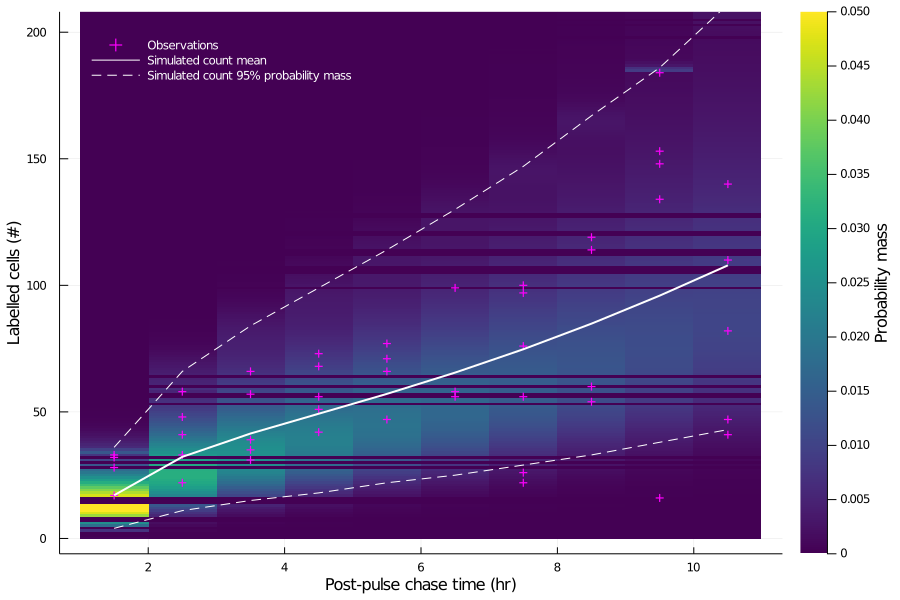
\includegraphics[width=1.\textwidth]{rys/a35sibMAP.png}}    
    \caption{{\bf \textit{rys} CMZ RPCs fail to contribute to the neural retina}}
    14\si{\micro\metre} coronal cryosections through representative sib (left panels) and \textit{rys} (right panels) eyes at 10dpf, 7 days after an 8hr BrdU pulse at 3dpf. Green: anti-BrdU labelling. Blue: Hoechst 33342 counterstain.
    Methods in \autoref{ssec:rysBrdUpulse}.
    \label{a35sibMAP}
\end{figure}

\begin{figure}[!h]
    \makebox[\textwidth][c]{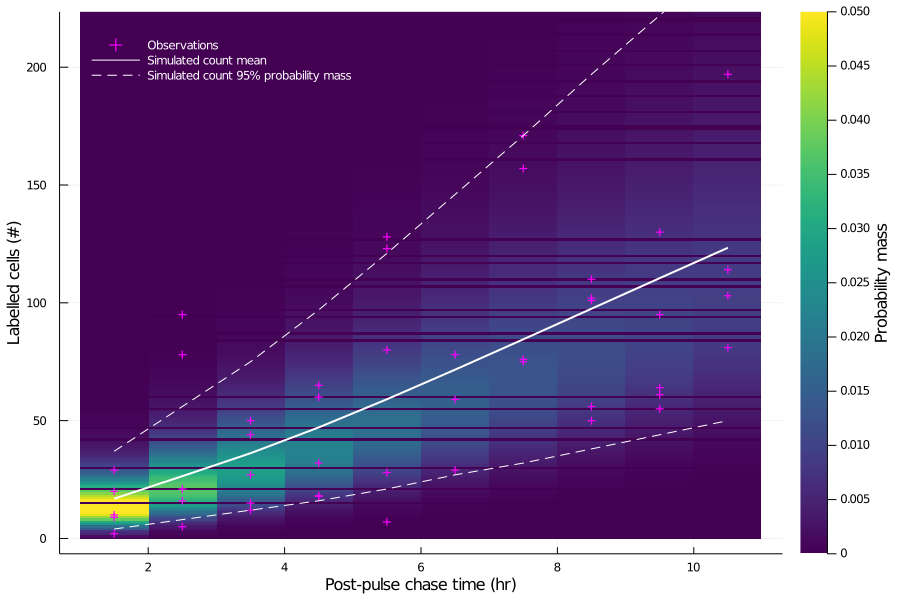
\includegraphics[width=1.\textwidth]{rys/a35rysMAP.png}}    
    \caption{{\bf MAP model output and observations for \textit{rys} mutant thymidine slice model of 5dpf cumulative EdU labelling}}
    Count of EdU-positive cells observed in 14\si{\micro\metre} coronal cryosections through \textit{rys} mutant CMZs at indicated chase times during a 10 mM EdU pulse (magenta crosses), overlaid with MAP model output. Probability mass distribution of the discrete non-parametric output is shown by color scale; yellow values include counts with >.05 mass. Output mean and 95\% mass are indicated by solid and dashed white lines.

    Methods in \autoref{ssec:rysBrdUpulse}.
    \label{a35rysMAP}
\end{figure}

\begin{sidewaysfigure}[!h]
    \makebox[\textwidth][c]{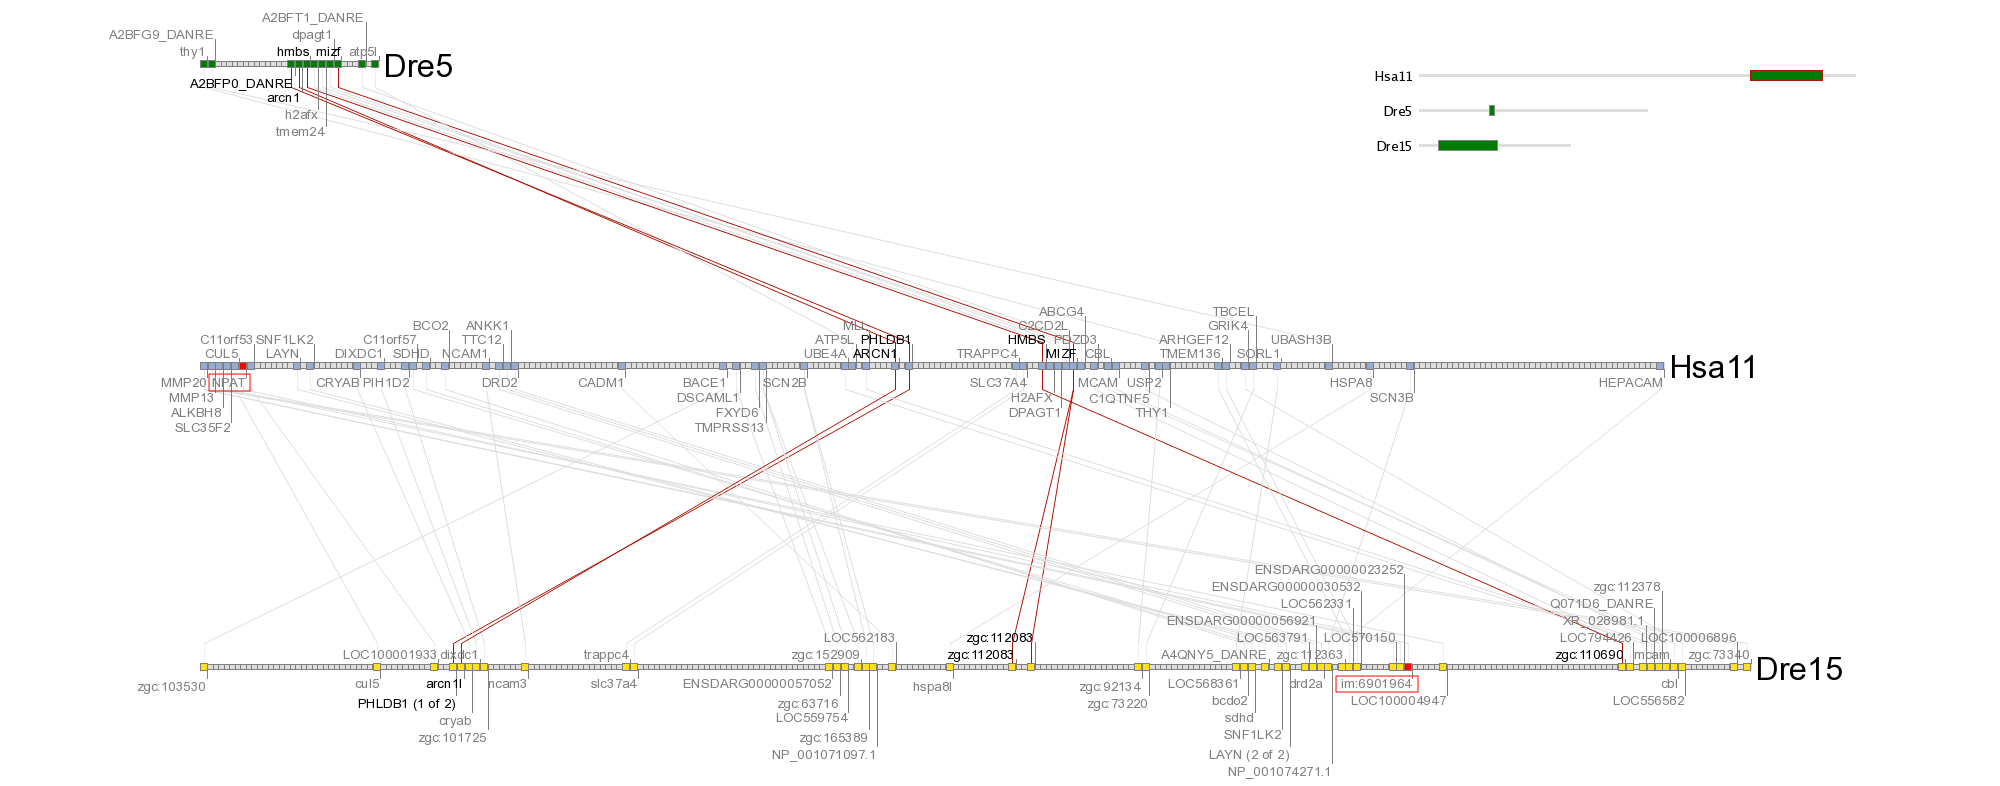
\includegraphics[width=1.2\textwidth]{rys/synteny2.png}}    
    \caption{{\bf Synteny Database output for the syntenic region containing \textit{D. rerio} npat}}
    Dre\#: \textit{Danio rerio chromosome \#}
    Hsa\#: \textit{Homo sapiens chromosome \#}

    The relative position of the displayed genomic neighbourhoods on their chromosome scaffolds is displayed inset, top right. \textit{D. rerio} npat is highlighted with a red square, visible on the right of the selected Dre15 region, annotated ``im:6901964''. \textit{H. sapiens} NPAT is highlighted similarly on the left of Hsa11. landmarks of the duplication and rearrangement event that brackets the position of npat on Dre15 are highlighted with red lines.

    On the scaffold of \textit{H. sapiens} chromosome 11, NPAT occurs upstream of the highlighted duplication cluster bracketed by ARCN1 and MIZF. Zebrafish npat is located in the midst of this rearranged, duplicated cluster, but does not appear to have been duplicated itself; at least if it was, no paralogue can be found by syntenic or similarity analysis.
    \label{synteny}
\end{sidewaysfigure}

\begin{figure}[!h]
    \makebox[\textwidth][c]{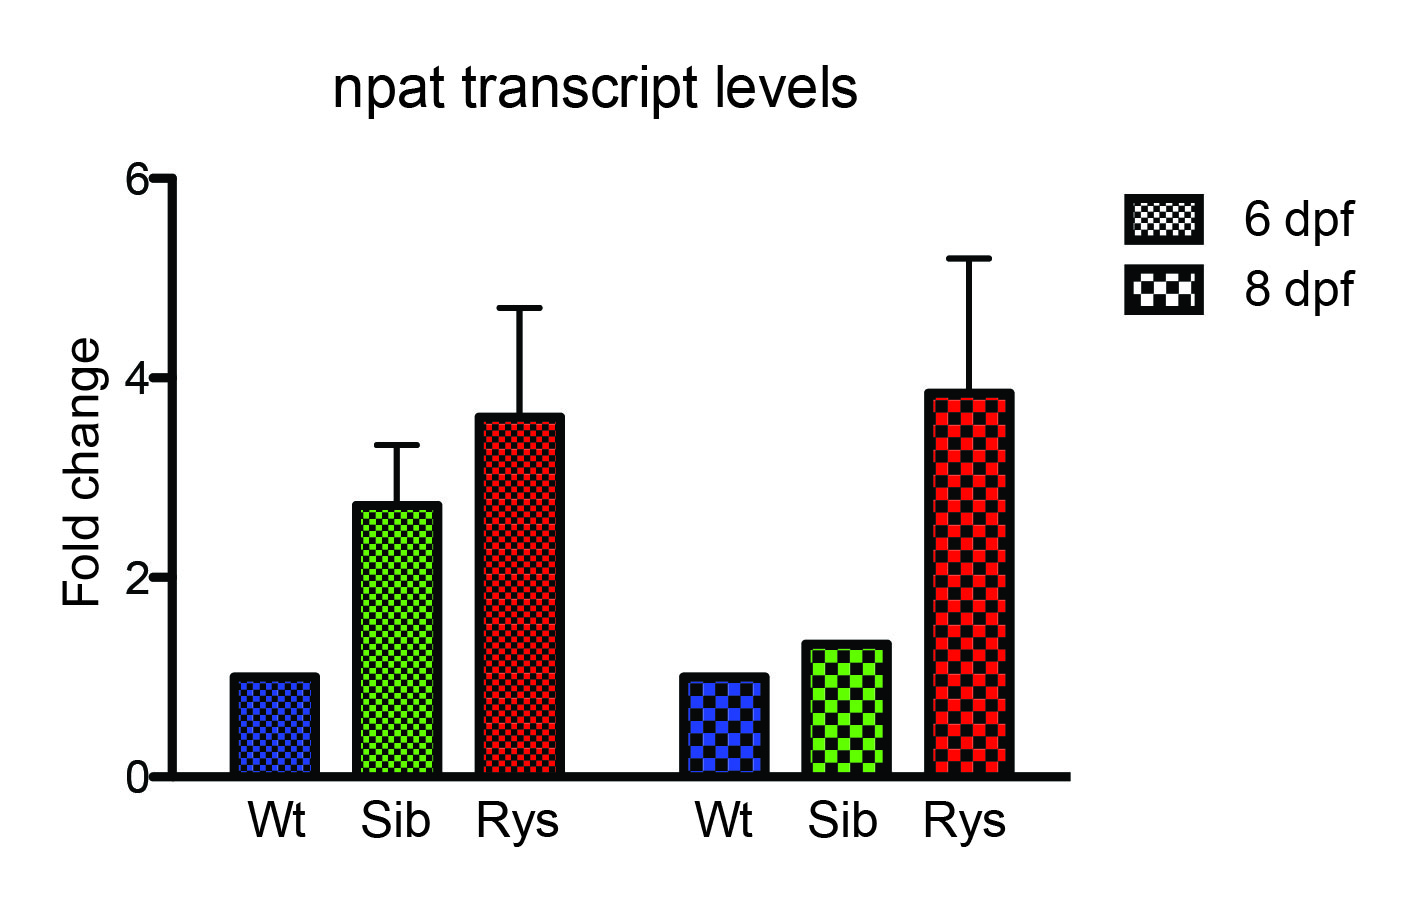
\includegraphics[width=1.\textwidth]{rys/npat transcripts.jpg}}    
    \caption{{\bf npat is overexpressed in \textit{rys}}} 
    \label{npatrtpcr}
\end{figure}

\begin{figure}[!h]
    \makebox[\textwidth][c]{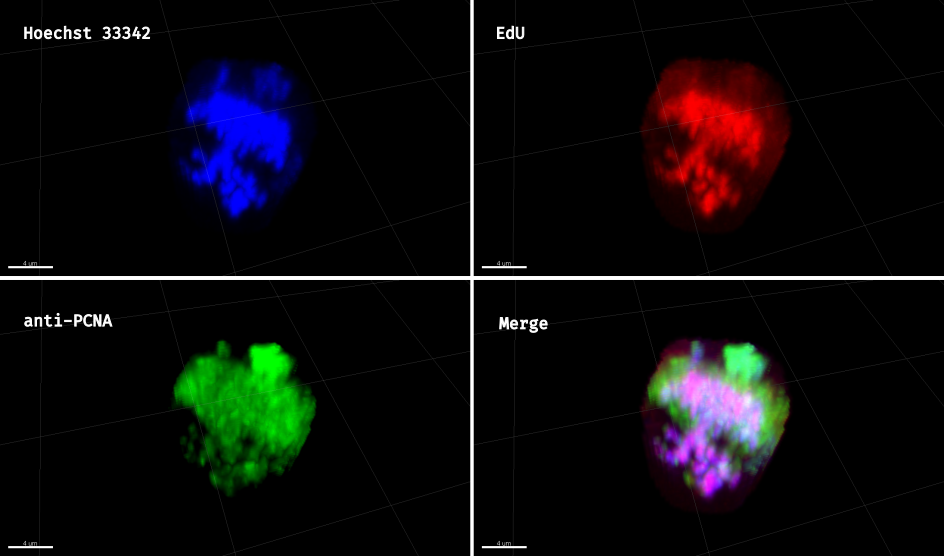
\includegraphics[width=1.\textwidth]{rys/mitosis.png}}    
    \caption{{\bf 10dpf mutant \textit{rys} RPCs are mitotic}} 3d volume reconstruction of a complete mitotic figure in a \textit{rys} mutant CMZ RPC at 10dpf, from a confocal micrograph of a 14\si{\micro\metre} coronal cryosection. Blue channel: Hoechst 33258; Green channel: PCNA; Red channel: EdU.
    \label{rysmitosis}
\end{figure}

\begin{figure}[!h]
    \makebox[\textwidth][c]{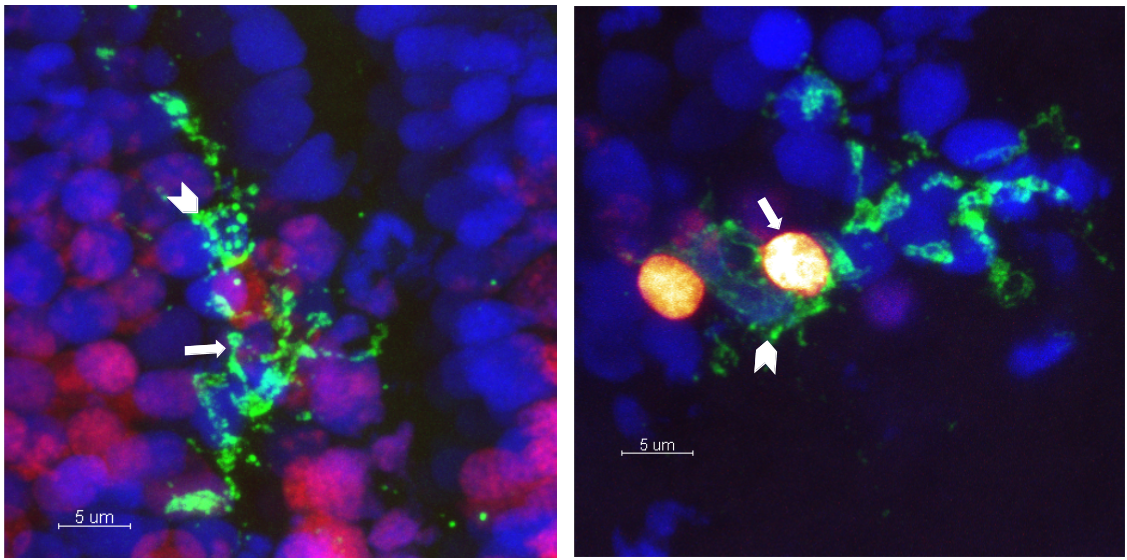
\includegraphics[width=1.\textwidth]{rys/rys_4c4.png}}    
    \caption{{\bf 4C4-positive microglia engulf \textit{rys} mutant RPCs}} 
    \label{phagocytosis}
\end{figure}


\begin{figure}[!h]
    \makebox[\textwidth][c]{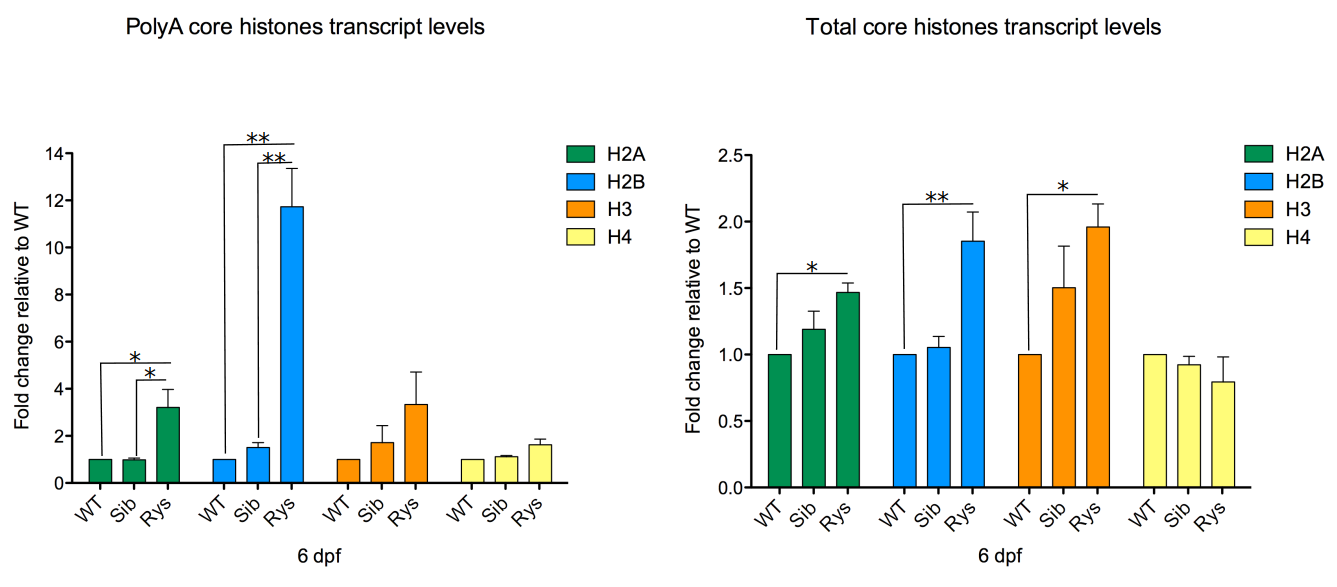
\includegraphics[width=1.\textwidth]{rys/morpholinoqPCR.png}}    
    \caption{{\bf Morpholinos directed to npat result in histone transcript overexpression similar to \textit{rys}}} 
    \label{morpholinoRTPCR}
\end{figure}

\begin{figure}[!h]
    \makebox[\textwidth][c]{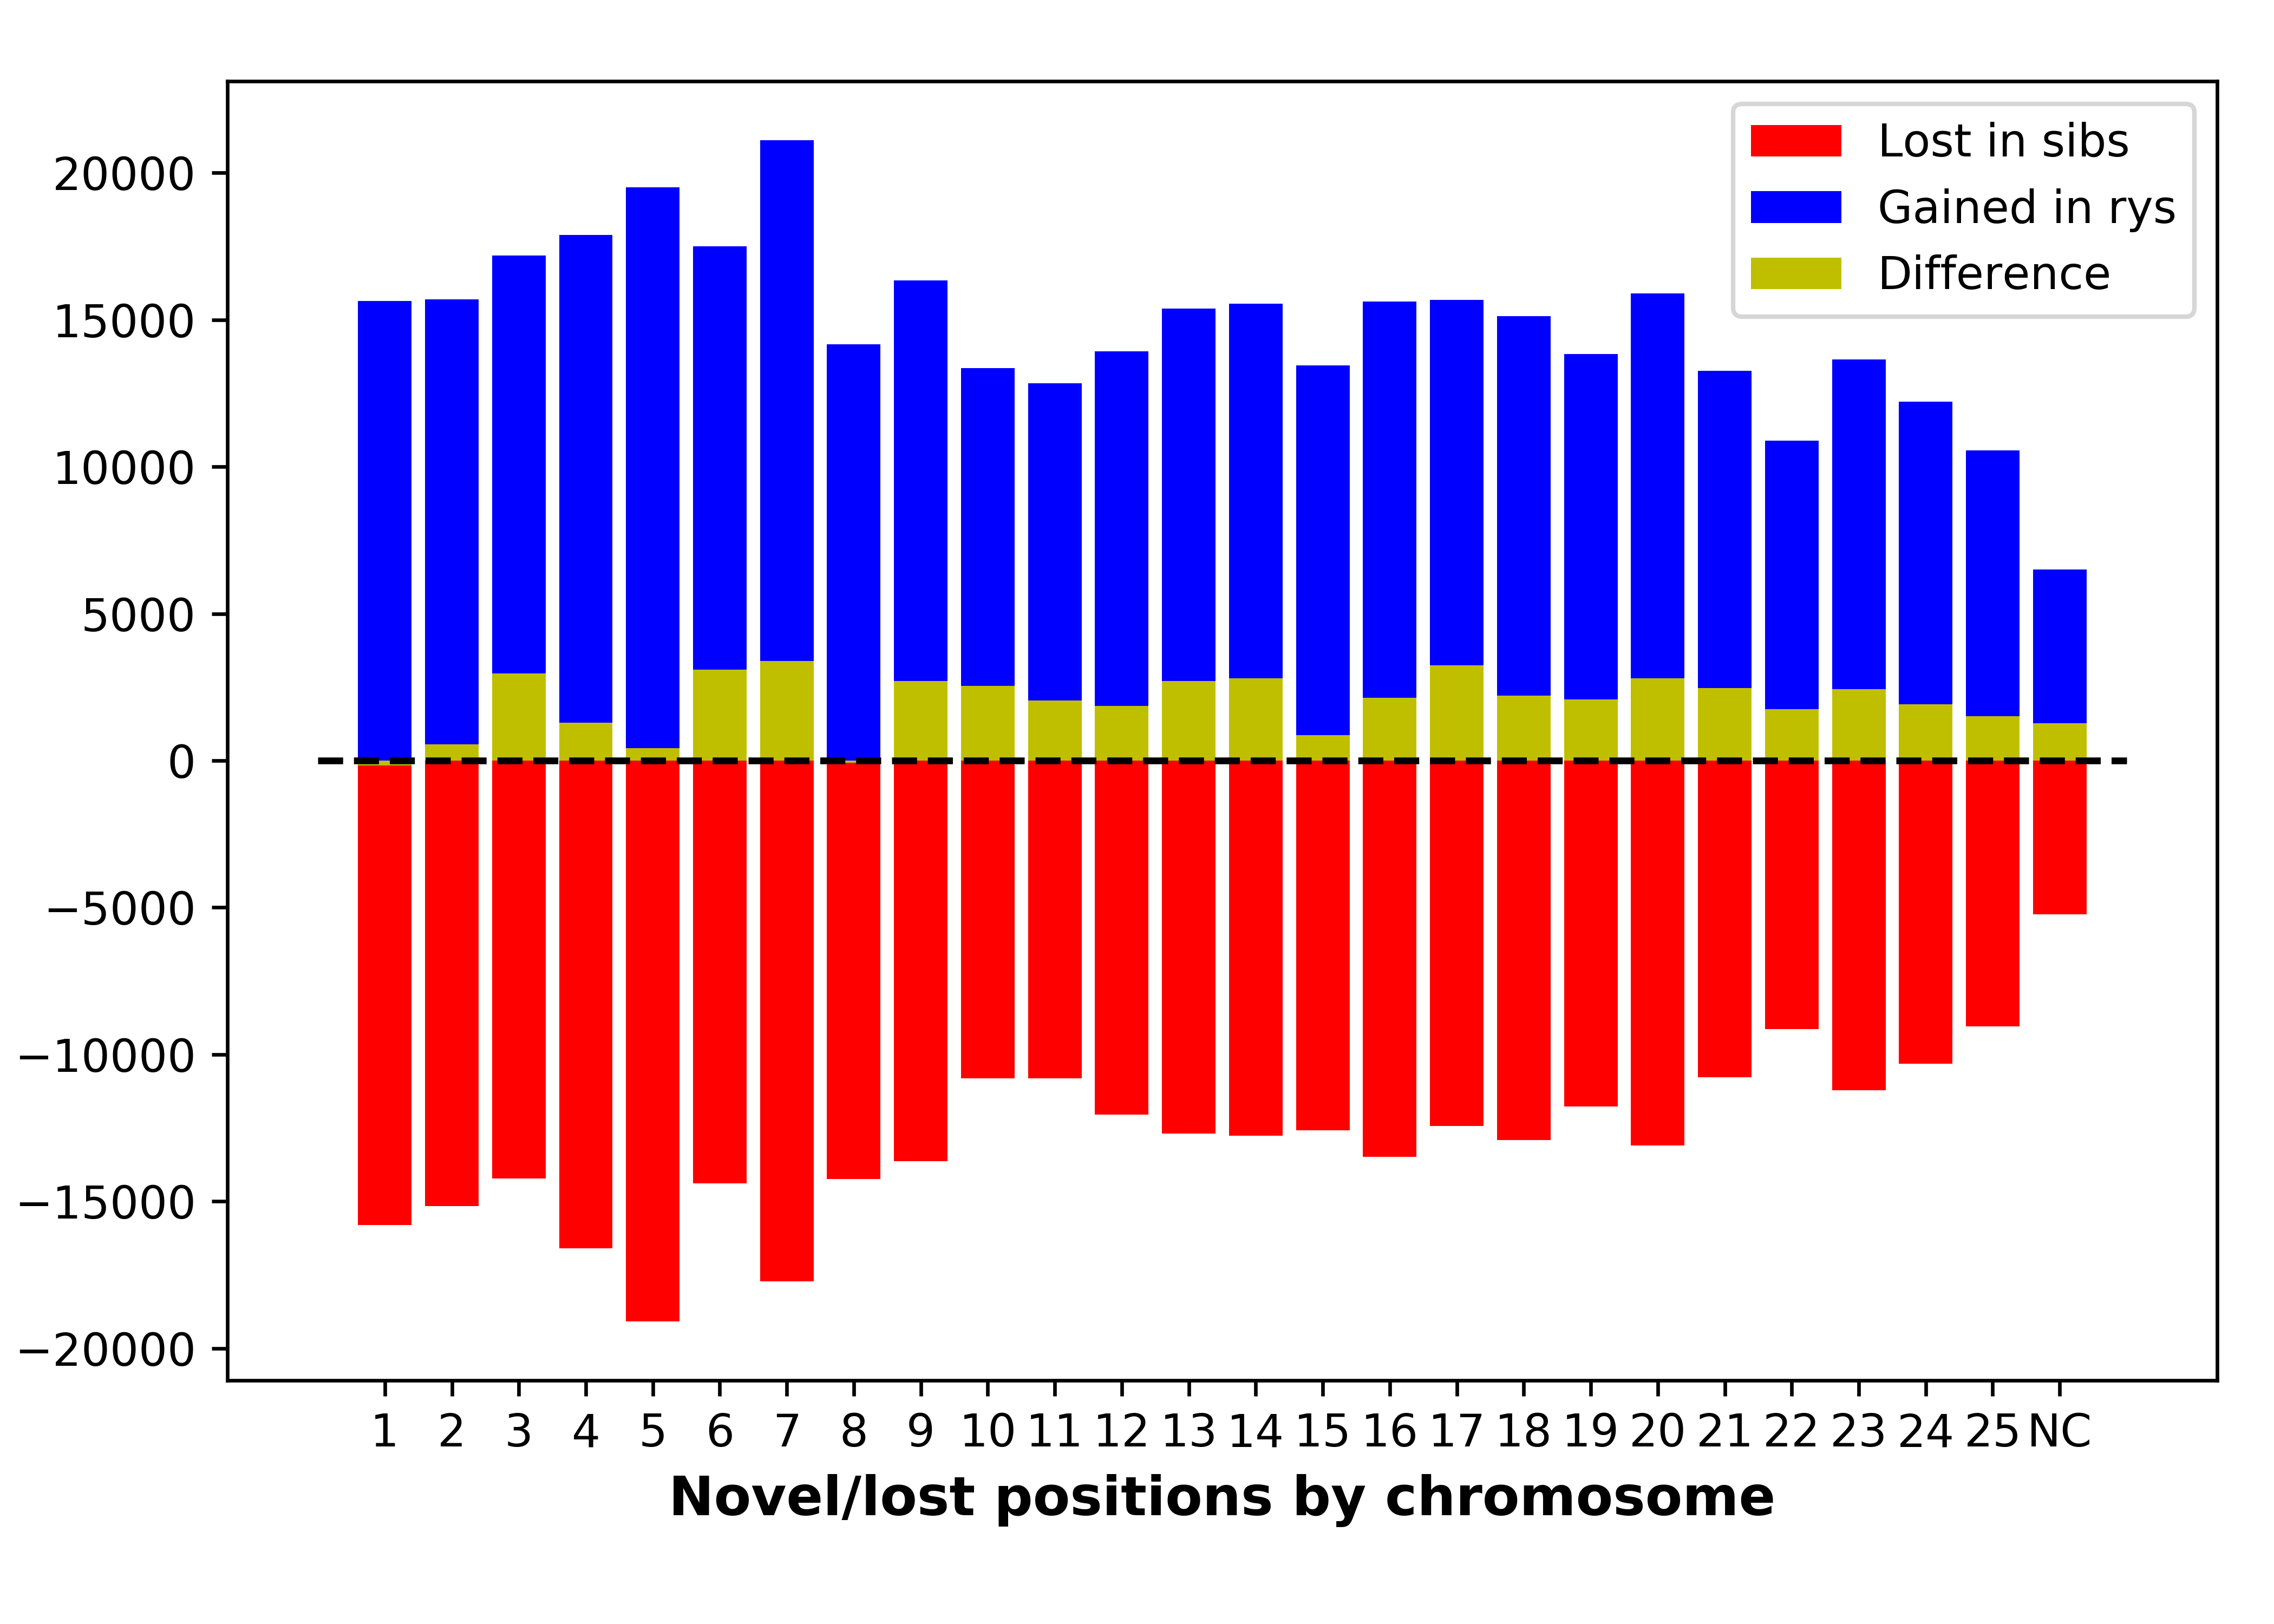
\includegraphics[width=.9\textwidth]{rys/chr_unique_positions.png}}    
    \caption{{\bf Novel nucleosome positions in \textit{rys} occur in similar numbers to those lost from sibs.}}
    Counts of positions found in sib but not \textit{rys} (red bars, represented as negative numbers, as these are `lost' in \textit{rys}) and those found in \textit{rys} but not sib (blue bars, `gained'). The magnitude of the difference between the counts is represented with a yellow bar.
    \label{diffposdist}
\end{figure}

\begin{figure}[!h]
    \makebox[\textwidth][c]{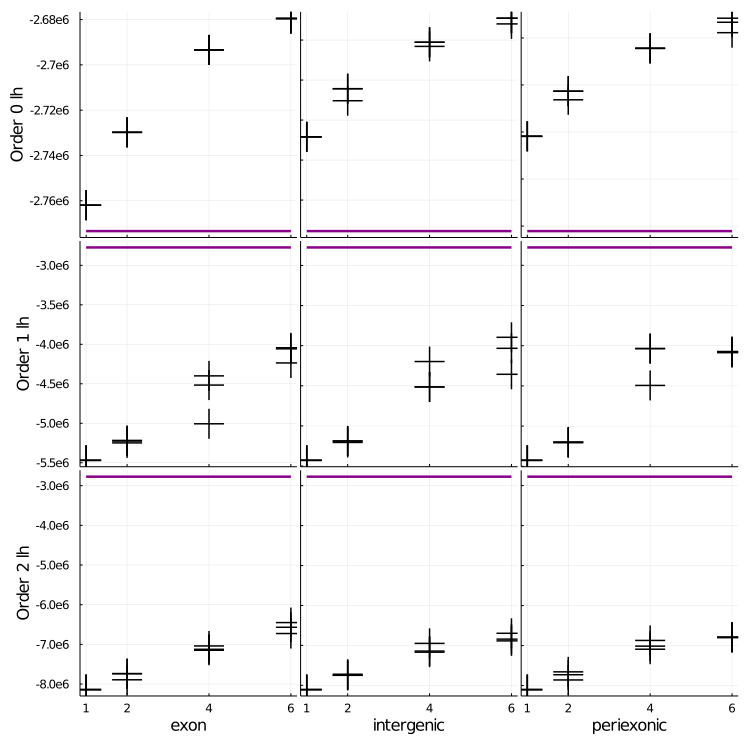
\includegraphics[width=.75\textwidth]{rys/bghmm.png}}    
    \caption{{\bf Test likelihoods for background HMMs trained on \textit{D. rerio} genome partitions}}
    \label{BHMMlh}
\end{figure}

\begin{figure}[!h]
    \makebox[\textwidth][c]{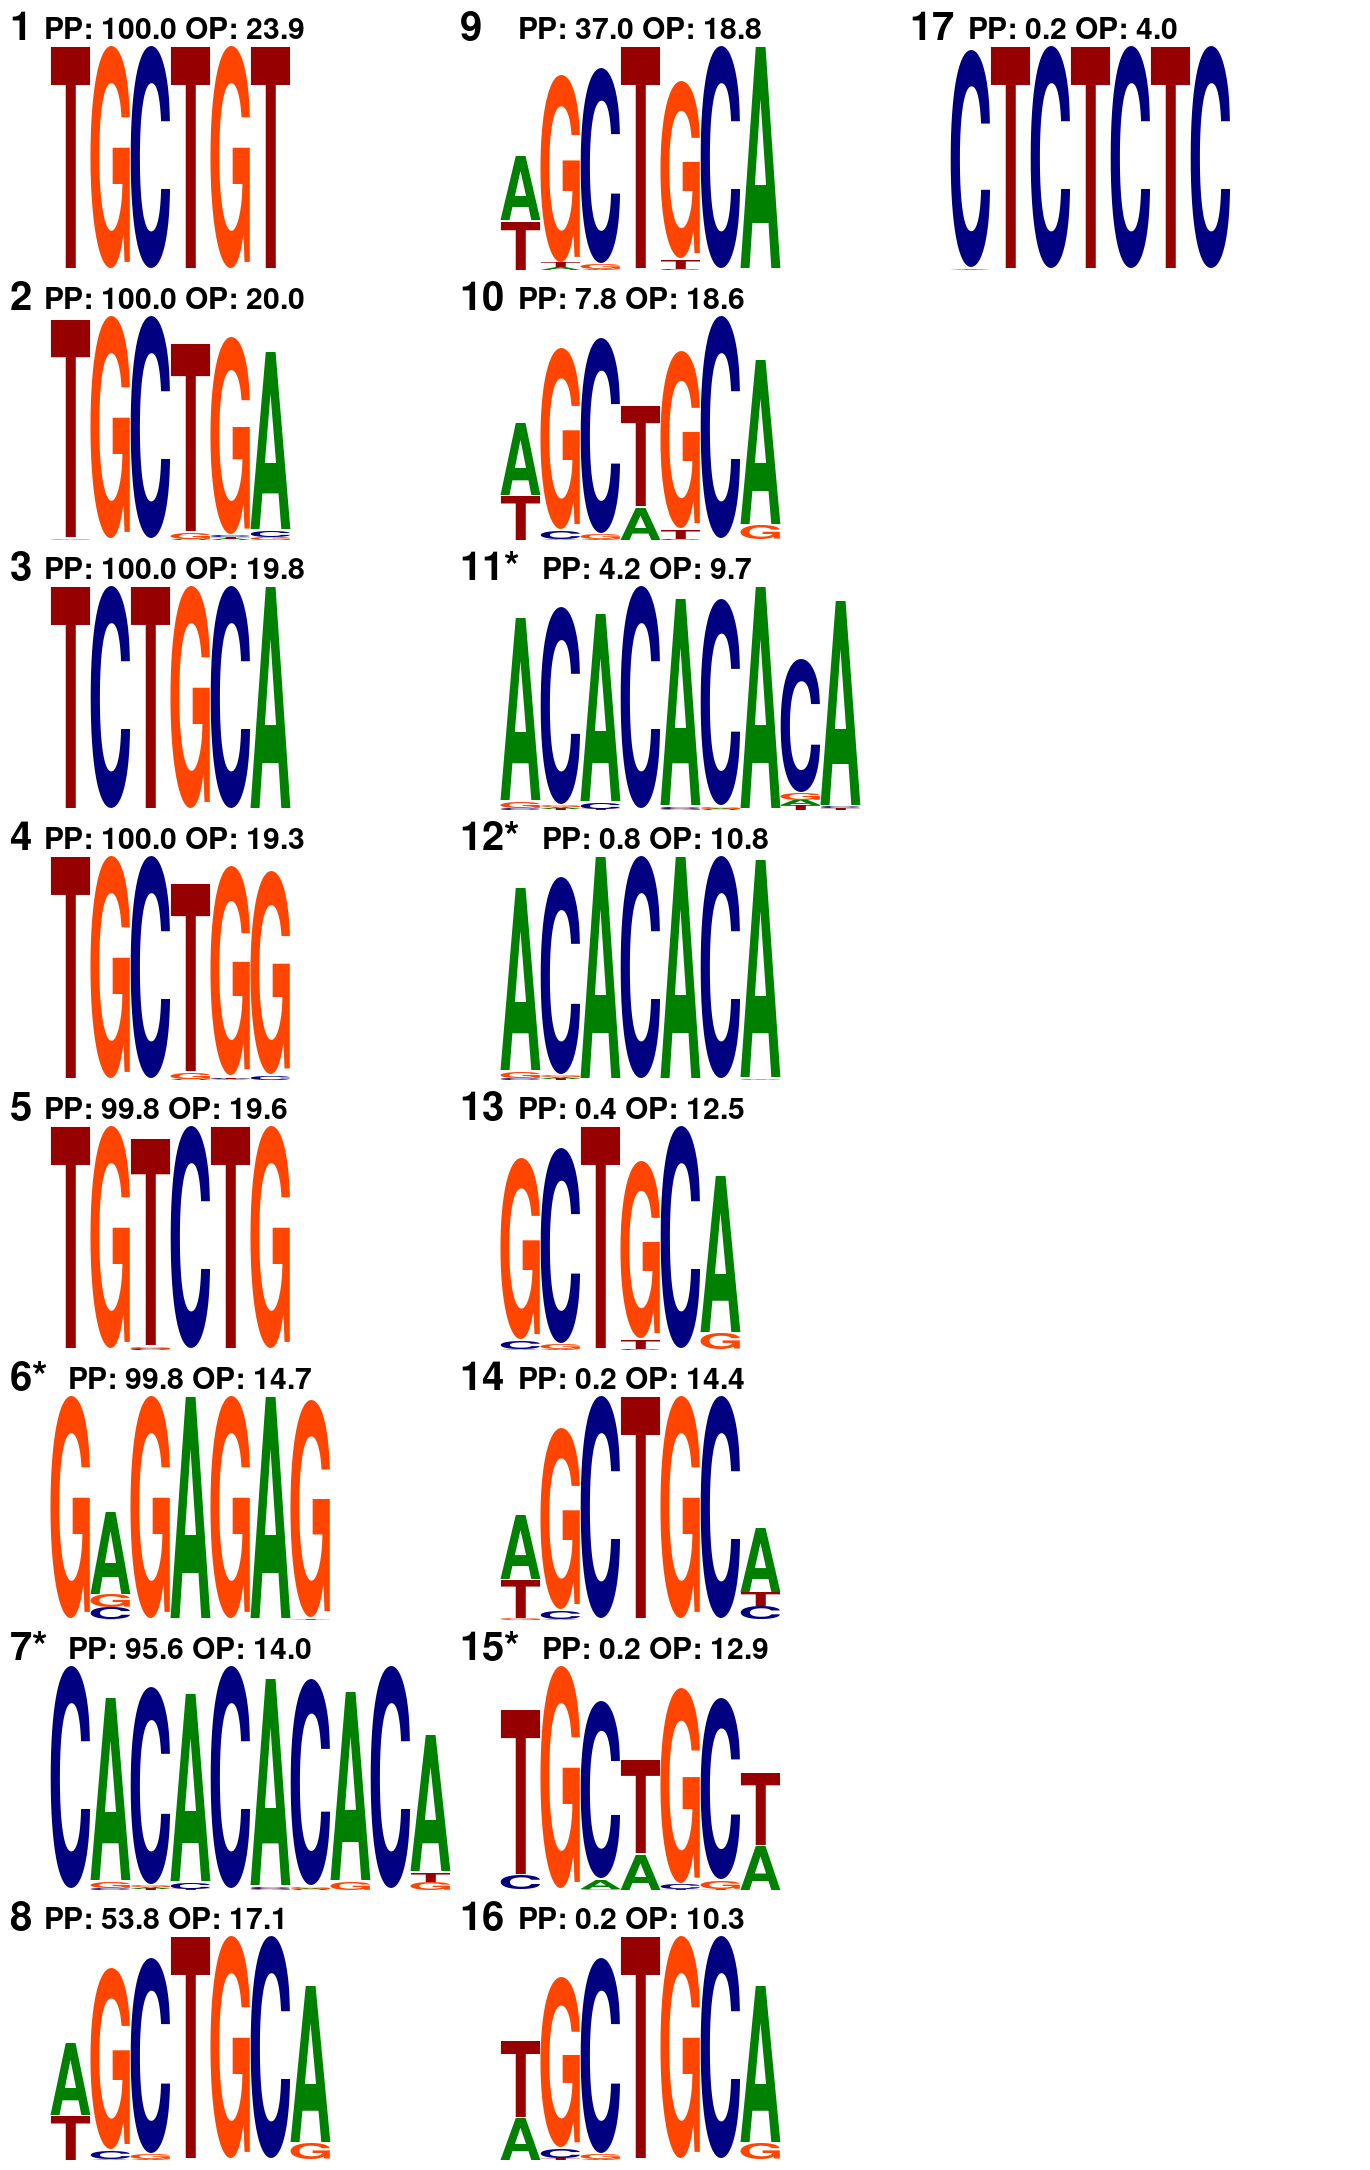
\includegraphics[width=.75\textwidth]{rys/combined_e_srcs.png}}    
    \caption{{\bf PWM sources detected in combined sib and rys differential sources.}}
    PWMs presented as sequence logos with letter height proportional to position informational content\/emission probability.
    
    PP: Posterior prevalence; proportion of models within the compressed maximum a posteriori ensemble which have this PWM as a signal source

    OP: Observation prevalence; mean proportion of observed position sequences this sequence is used to explain, over all posterior samples
    \label{combinedmotifs}
\end{figure}

\FloatBarrier

\section{Supplementary tables}

\begin{table}[!ht]
    \caption{Evidence for Normal vs. Log-Normal models of layer and lineage contribution}
    \begin{tabular}{|l|l|l|l|l|l|} 
        \hline
        {\bf Morpholino} & {\bf Measurement} & {\bf Separate logZ} & {\bf Combined logZ} & {\bf logZR} & {\bf $\sigma$ sign.}\\ \hline \hline
        ATG & CMZ pop. & -236.4 ± 2.3 & {\bf -198.3 ± 2.2} & -38.1 ± 3.2 & 12.1 \\ \hline
        ATG & Total sectional pop. & -412.4 ± 7.8 & {\bf -225.3 ± 4.9} & -187.1 ± 9.2 & 20.3 \\ \hline
        ATG & Sectional pop. per CMZ cell & {\bf -70.18 ± 0.86} & -78.0 ± 0.86 & 7.8 ± 1.2 & 6.4 \\ \hline
        ATG & Dorsal CMZ pop. & -169.5 ± 1.4 & {\bf -151.75 ± 0.8} & -17.8 ± 1.6 & 11.2 \\ \hline
        ATG & Ventral CMZ pop. & -223.1 ± 1.5 & {\bf -165.3 ± 1.0} & -57.8 ± 1.8 & 32.5 \\ \hline
        ATG & Nuclear volume & -290.6 ± 1.8 & {\bf -192.7 ± 1.8} & -97.9 ± 2.5 & 39.6 \\ \hline
        ATG & Nuclear sphericity & {\bf -186.13 ± 0.79} & -215.66 ± 0.57 & 29.53 ± 0.97 & 30.3 \\ \hline
        Spl & CMZ pop. & -272.6 ± 2.4 & {\bf -197.0 ± 2.6} & -75.7 ± 3.6 & 21.2 \\ \hline
        Spl & Total sectional pop. & -455.9 ± 8.3 & {\bf -205.6 ± 4.7} & -250.3 ± 9.5 & 26.3 \\ \hline
        Spl & Sectional pop. per CMZ cell & -87.04 ± 0.17 & {\bf -66.22 ± 0.29} & -20.82 ± 0.34 & 62.0 \\ \hline
        Spl & Dorsal CMZ pop. & -226.2 ± 1.7 & {\bf -171.0 ± 1.1} & -55.2 ± 2.0 & 27.7 \\ \hline
        Spl & Ventral CMZ pop. & -234.97 ± 0.81 & {\bf -222.3 ± 1.7} & -12.7 ± 1.9 & 6.8 \\ \hline
        Spl & Nuclear volume & -277.5 ± 1.6 & {\bf -223.2 ± 2.1} & -54.3 ± 2.7 & 20.4 \\ \hline
        Spl & Nuclear sphericity & -94.3 ± 1.1 & {\bf -67.71 ± 0.39} & -26.6 ± 1.1 & 23.2 \\ \hline
    \end{tabular}
   
    \begin{flushleft}logZ: logarithm of p(D), the marginal likelihood of the data, or model evidence.  Largest evidence values bolded. logZR: evidence ratio; positive values in favour of stable model.
    \end{flushleft}
    \label{morpholinoev}
\end{table}
